%%=============================================================================
%% Methodologie
%%=============================================================================

\chapter{\IfLanguageName{dutch}{Methodologie}{Methodology}}%
\label{ch:methodologie}
\section{Dataverwerking}
\subsection{Technologieën voor databases}
In het eerste deel van deze bachelorproef wordt een literatuurstudie uitgevoerd over de verschillende technologieën die worden gebruikt om data op te slaan en te verwerken.
De werking en efficiëntie van Cosmos DB zijn onderzocht, evenals de werking van de Gremlin API en de toepassing ervan bij het opzetten van een grafiekmodel.
De ontvangen data is vrij complex en betreft een boomstructuur uit SAP, aangeleverd via een JSON-bestand.
Het lastigste aan deze data is de interpretatie van de verschillende sleutel-waardeparen en de hiërarchie, die niet volledig klopt, waardoor de juiste verdeling tussen afdeling en machine moeilijk vast te stellen was.
Elke sleutel heeft een specifieke betekenis en waarde die vertaald moet worden naar een leesbare vorm voor het grafiekmodel.
Na het verwerken, begrijpen en opschonen van de data is deze omgezet naar JSON-LD-formaat volgens de GS1-standaarden.
Vanaf dat moment is de data klaar om te worden ingeladen in Cosmos DB.\@
Met behulp van Python en JavaScript kunnen grote delen van het proces geautomatiseerd worden, wat zorgt voor een snellere en efficiëntere werkwijze.

\section{Proof of concept}
\subsection{Opzetten van een grafiekmodel}
In het tweede deel van deze bachelorproef wordt een proof of concept opgesteld van het grafiekmodel waarbij de SAP-data van ArcelorMittal Gent wordt gebruikt.
Zoals eerder vermeld, is de JSON-data omgezet naar GS1-standaarden in een JSON-LD-bestand. Dit bestand, opgemaakt met schema.org en GS1 EPCIS-events, wordt ingeladen in Cosmos DB via NodeJS en de Gremlin API.\@
Hierdoor ontstaat een grafiekmodel waarin de data gevisualiseerd en geanalyseerd kan worden aan de hand van de relaties tussen de verschillende producten en processen.
Dit grafiekmodel kan worden gevisualiseerd met behulp van Graph Explorer, dat ingebouwd is in Azure Cosmos DB, of met andere visualisatietools.
In figuur~\ref{fig:chatbot_workflow} is een voorbeeld te zien van de werking van de chatbot.
In het eerste deel van de figuur wordt getoond wat er moet gebeuren met de data als deze nog niet in JSON-LD-formaat is.
In het tweede deel wordt weergegeven hoe de chatbot van een vraag tot een antwoord komt.

\subsection{Opzetten van een chatbot}
In het derde deel van deze bachelorproef wordt een chatbot opgesteld die de data van het grafiekmodel kan bevragen en analyseren.
De input van dit model is een vraag van de gebruiker; deze wordt vertaald naar een Gremlin-query die de data in Cosmos DB beantwoordt.
De query zoekt vervolgens de relevante knopen en relaties, die verwerkt en geformatteerd worden tot leesbare tekst.
De chatbot werkt iteratief: in de eerste stap wordt de query gemaakt, in de tweede stap worden de resultaten teruggegeven aan de gebruiker.
Tijdens dit proces wordt gebruikgemaakt van een Retrieval Augmented Generation (RAG)-model dat de resultaten van de Gremlin-query kan verwerken en formatteren naar leesbare tekst.
Er zijn twee methoden om een query op te halen. De eerste methode maakt gebruik van Elasticsearch, dat in een Docker-container draait.
Hiervoor wordt een JSON-bestand met voorbeeldvragen gebruikt, geïndexeerd in een database, om sneller en nauwkeuriger de juiste query te vinden.
De tweede methode maakt gebruik van een Large Language Model (LLM) wanneer er geen bijpassende query in Elasticsearch gevonden wordt.
Daarnaast wordt de query die van het LLM terugkomt gevalideerd, zodat deze uitvoerbaar is in Cosmos DB.\@

Docker wordt ingezet om de verschillende componenten van de chatbot te beheren en te laten communiceren.
Hierdoor kan de chatbot eenvoudig worden opgezet en beheerd, zonder zorgen over de onderliggende infrastructuur.
In figuur~\ref{fig:output} is een voorbeeld te zien van de output van de chatbot.

\begin{figure}[H]
    \centering
    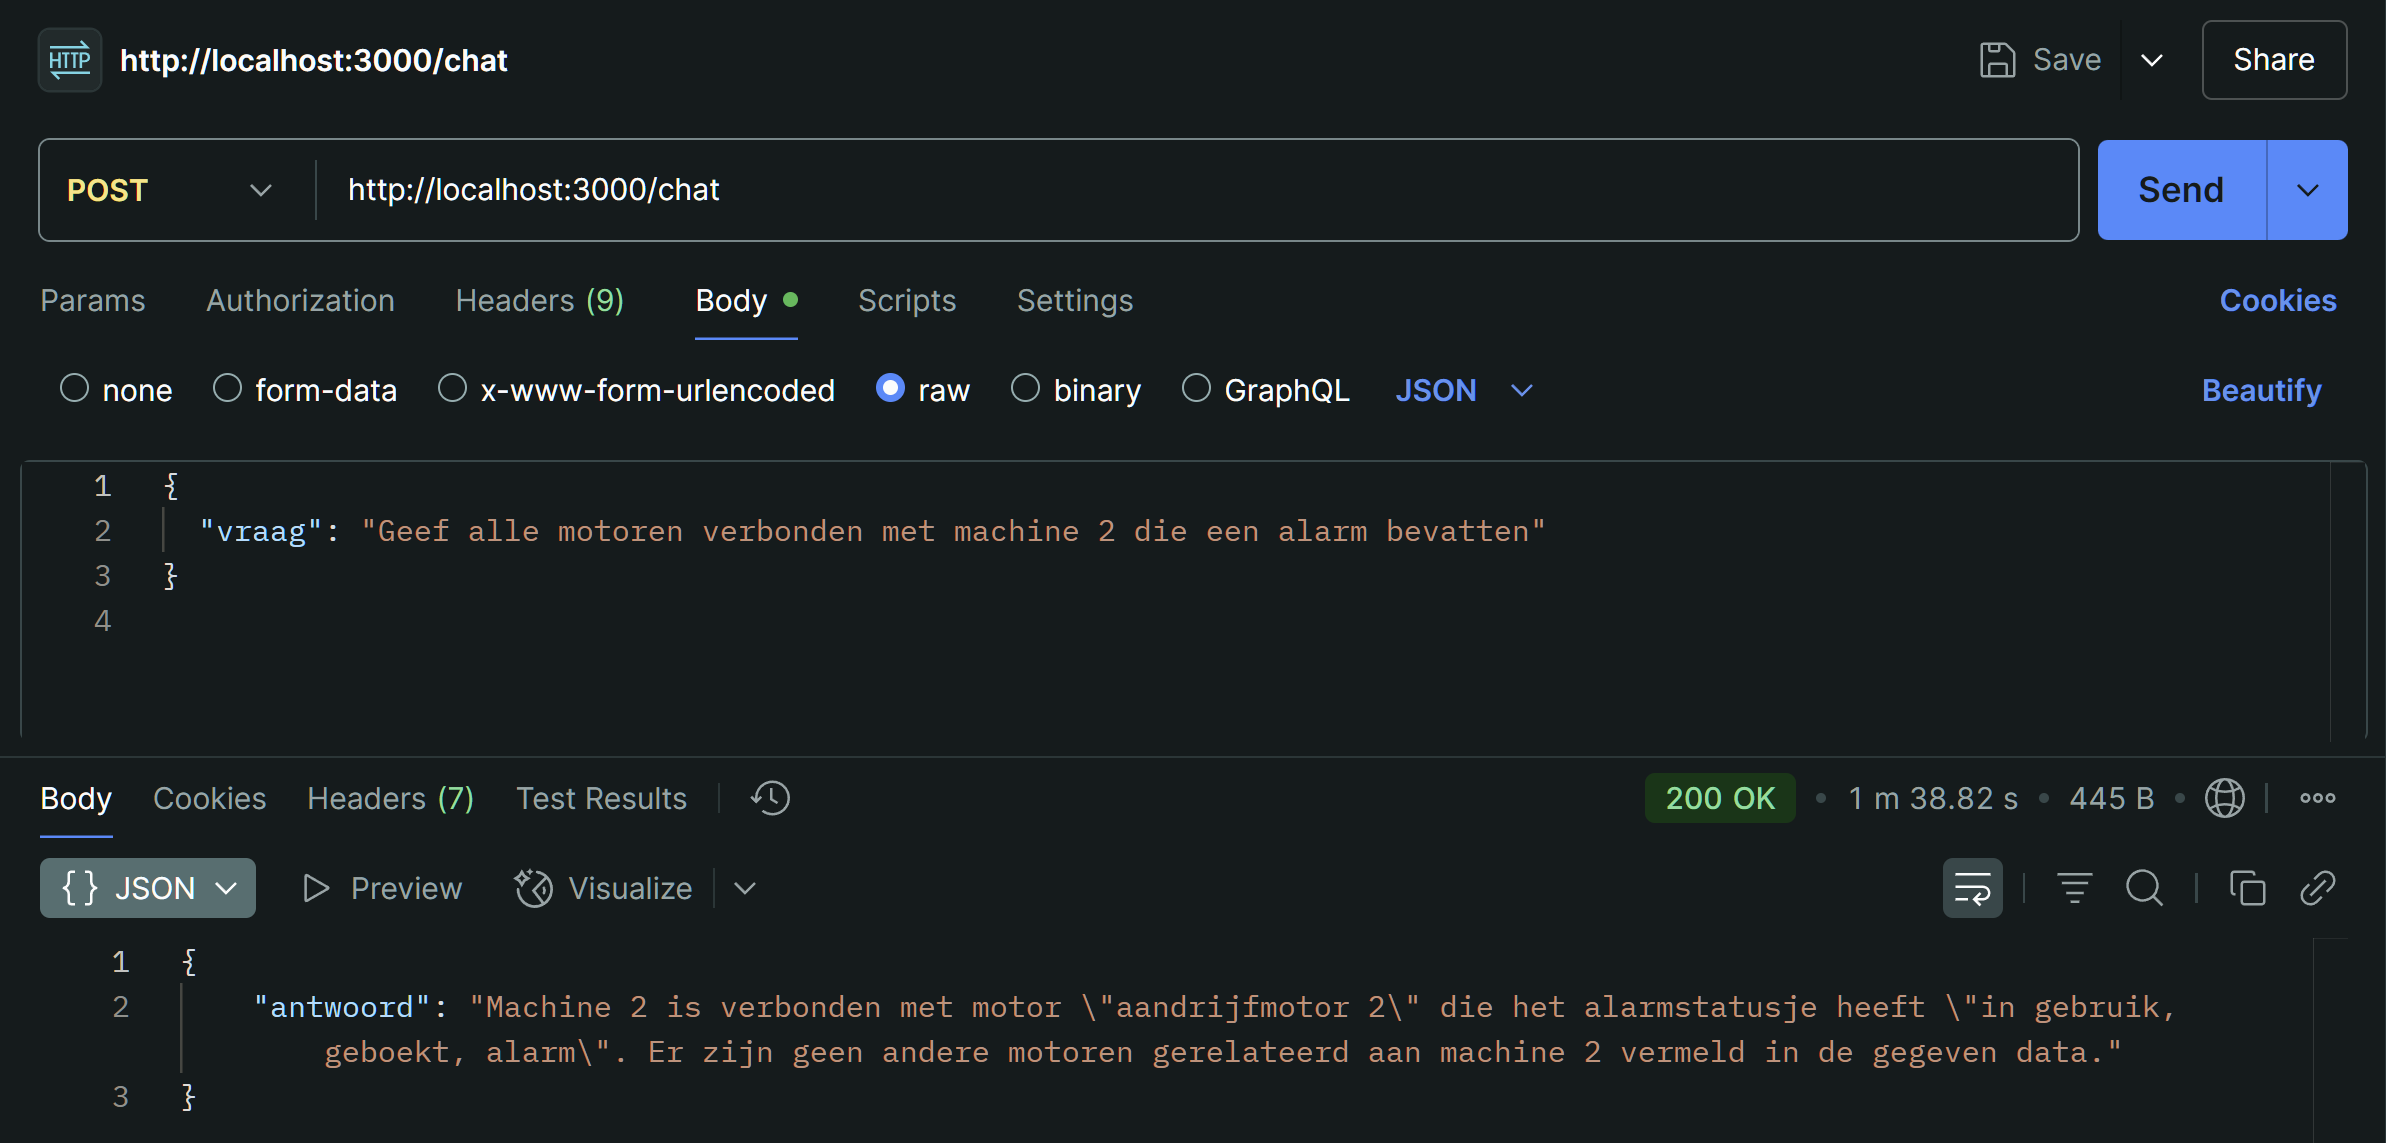
\includegraphics[width=0.8\textwidth]{./img/response.png}
    \caption[Output chatbot]{\label{fig:output}Voorbeeld van output op basis van Cosmos DB.}
\end{figure}

\subsection{Structuur chatbot}
Voor de chatbot wordt er gebruik gemaakt van CodeLlama voor het genereren van een Gremlin-query en een Phi4-model voor het samenvatten van data uit de database.
Deze modellen worden via Ollama in een Docker-container gebruikt, zodat er een lokale versie kan draaien die niet verbonden is met het internet. Dit wordt gedaan omdat er zekerheid moet zijn dat het model geen data via het internet opslaat, bijvoorbeeld om het eigen model verder te trainen.
Een voorbeeld van een model dat zichzelf traint is OpenAI, dat getraind is op een grote dataset waarbij deze data ook wordt gebruikt om het model te verbeteren.
Dit is niet de bedoeling voor ons model, omdat er zeker geen datalek mag worden veroorzaakt.
Met de chatbot kunnen vragen beantwoord worden die gerelateerd zijn aan het productieproces van ArcelorMittal Gent, zoals: \emph{``Welke fabrieken staan er in Gent\texttt{?}''} of \emph{``Geef alle kranen met een melding op de motor''.}
Dit probleem wordt opgelost met het iteratieve proces binnen onze chatbot, waarbij de vraag wordt doorgegeven aan de chatbot om beantwoord te worden.

%% TODO: In dit hoofstuk geef je een korte toelichting over hoe je te werk bent
%% gegaan. Verdeel je onderzoek in grote fasen, en licht in elke fase toe wat
%% de doelstelling was, welke deliverables daar uit gekomen zijn, en welke
%% onderzoeksmethoden je daarbij toegepast hebt. Verantwoord waarom je
%% op deze manier te werk gegaan bent.
%% 
%% Voorbeelden van zulke fasen zijn: literatuurstudie, opstellen van een
%% requirements-analyse, opstellen long-list (bij vergelijkende studie),
%% selectie van geschikte tools (bij vergelijkende studie, "short-list"),
%% opzetten testopstelling/PoC, uitvoeren testen en verzamelen
%% van resultaten, analyse van resultaten, ...
%%
%% !!!!! LET OP !!!!!
%%
%% Het is uitdrukkelijk NIET de bedoeling dat je het grootste deel van de corpus
%% van je bachelorproef in dit hoofstuk verwerkt! Dit hoofdstuk is eerder een
%% kort overzicht van je plan van aanpak.
%%
%% Maak voor elke fase (behalve het literatuuronderzoek) een NIEUW HOOFDSTUK aan
%% en geef het een gepaste titel.



